\documentclass[a4paper]{scrartcl}
\usepackage[cm]{fullpage}
\usepackage{amsmath, amssymb}
\usepackage{siunitx}

\usepackage{tikz, pgfplots}
\tikzstyle{every node} = [align = center]
\pgfplotsset{
    compat = 1.9,
    bfield/.style = {
        axis lines = middle,
        grid = both,
        minor tick num = 3,
        every major grid/.style = {orange, opacity=0.5},
        clip = false,
        xlabel = Current (\si{\ampere}),
        ylabel = B-field (\si{\milli\tesla}),
        legend pos = outer north east
    },
    bfield-scatter/.style = {
        only marks,
        error bars/.cd,
        x dir = both, y dir = both,
        x explicit, y explicit
    }
}

\begin{document}

\title{PHYS1241: Magnetic Fields and the ``Slinky'' Coil}
\author{ \\ \\ }
\date{2015-09-03}
\maketitle

\section{Abstract}

\section{Introduction}

\section{Materials and Methods}
Please refer to pages 91 to 94 inclusive in the PHYS1241 laboratory manual for the base materials and methods used.

Since the magnetic field sensor has a systematic zero error of \(\varepsilon\), we can measure the field once in the positive direction \(B_+ = \varepsilon + B\) and once in the negative direction \(B_- = \varepsilon - B\), and use these values to calculate the true value for \(B\):
\begin{align*}
    \frac{B_+ - B_-}{2} &= \frac{\varepsilon + B - \varepsilon + B}{2} \\
    &= B
\end{align*}

For part 2, measurements were taken at the middle and the ends of the slinky. The slinky was held constant at 34 loops at \SI{100 \pm 1}{\centi\metre} and then \SI{50 \pm 1}{\centi\metre}, giving \SI{34}{} and \SI{68 \pm 1}{loops per metre}, respectively.

Part 3 was done with the slinky at 38 loops in \SI{50 \pm 1}{\centi\metre}, giving \SI{76 \pm 2}{loops per metre}. There was no need to account for the systematic zero error in the magnetic field probe due to only requiring the change in B-field strength to calculate \(\mu_0 n = \frac{B}{I}\), so only \(B_-\) was measured.

\section{Results}
\subsection{Part 1: The Magnetic Field of the Earth}
\begin{table}
    \centering
    \begin{tabular}{c | c | c | c}
        Orientation & \(B_+\) (\si{\milli\tesla}) & \(B_-\) (\si{\milli\tesla}) & \(B\) (\si{\milli\tesla}) \\
        \hline
        Horizontal & \SI{0.011 \pm 0.004}{} & \SI{-0.044 \pm 0.004}{} & \SI{0.023 \pm 0.003}{} \\
        Vertical & \SI{0.031 \pm 0.004}{} & \SI{-0.075 \pm 0.004}{} & \SI{0.053 \pm 0.003}{} \\
        \hline
    \end{tabular}
    \caption{Part 1 raw data and inferred \(B\)}
    \label{tab:part1_data}
\end{table}

Along with the data recorded in Table \ref{tab:part1_data}, a maxima in the field strength was found to be at a \SI{70 \pm 10}{\degree} inclination. Using the horizontal and vertical components from the data, the inclination can also be calculated to equal \SI{67 \pm 3}{\degree} and \SI{0.058 \pm 0.003}{\milli\tesla}.

\subsection{Part 2: The Magnetic Field of the Slinky}
\begin{table}
    \centering
    \begin{tabular}{c | c | c | c | c}
        Length (\si{\centi\metre}) & Current (\si{\ampere}) & Middle (\si{\milli\tesla}) & End 1 (\si{\milli\tesla}) & End 2 (\si{\milli\tesla}) \\
        \hline
        \SI{100 \pm 1}{} & \SI{2.4 \pm 0.2}{} & \SI{0.130 \pm 0.003}{} & \SI{0.122 \pm 0.003}{} & \SI{0.134 \pm 0.003}{} \\
        \SI{100 \pm 1}{} & \SI{4.7 \pm 0.2}{} & \SI{0.246 \pm 0.003}{} & \SI{0.223 \pm 0.003}{} & \SI{0.246 \pm 0.003}{} \\
        \SI{50 \pm 1}{} & \SI{4.7 \pm 0.4}{} & \SI{0.459 \pm 0.003}{} & \SI{0.424 \pm 0.003}{} & \SI{0.336 \pm 0.003}{} \\
        \hline
    \end{tabular}
    \caption{Part 2 raw data after removing the zero error}
    \label{tab:part2_data}
\end{table}

\begin{figure}
    \centering
    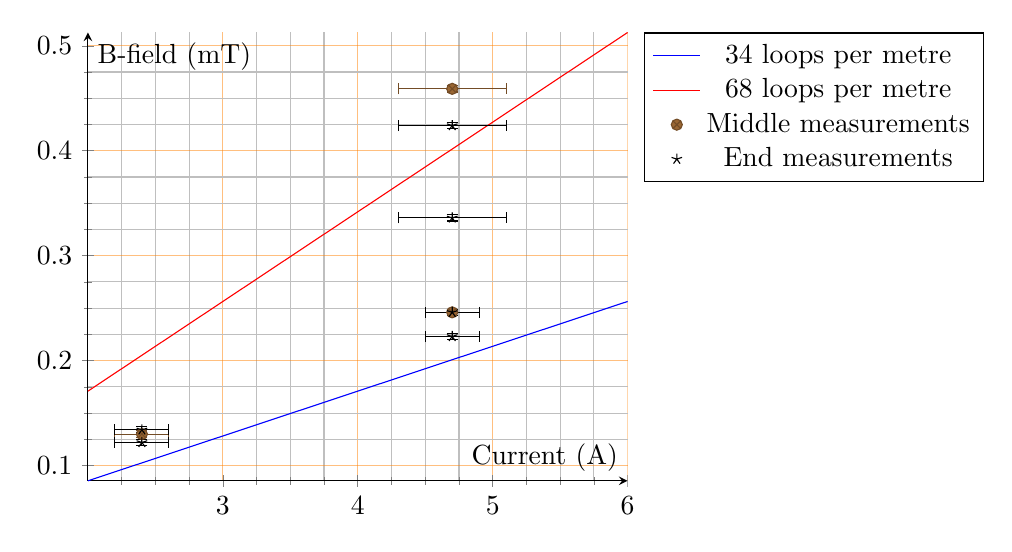
\begin{tikzpicture}
        \begin{axis}[bfield]
            \addplot +[no marks, domain = 2:6] {1000 * 4 * pi * 10^(-7) * 34 * x};
            \addlegendentry{34 loops per metre}
            
            \addplot +[no marks, domain = 2:6] {1000 * 4 * pi * 10^(-7) * 68 * x};
            \addlegendentry{68 loops per metre}

            \addplot +[bfield-scatter] table [
                x error = xerror,
                y error = yerror
            ] {
                x   y       xerror  yerror
                2.4 0.130   0.2     0.003
                4.7 0.246   0.2     0.003
                4.7 0.459   0.4     0.003
            };
            \addlegendentry{Middle measurements}
            
            \addplot +[bfield-scatter] table [
                x error = xerror,
                y error = yerror
            ] {
                x   y       xerror  yerror
                2.4 0.122   0.2     0.003
                2.4 0.134   0.2     0.003
                4.7 0.223   0.2     0.003
                4.7 0.246   0.2     0.003
                4.7 0.424   0.4     0.003
                4.7 0.336   0.4     0.003
            };
            \addlegendentry{End measurements}
        \end{axis}
    \end{tikzpicture}
    \caption{Part 2 raw data compared to the predicted values}
    \label{fig:part2_graph}
\end{figure}

Table \ref{tab:part2_data} lists the collected data points after removing the systematic error by using the same method as part 1. Figure \ref{fig:part2_graph} plots these points against the predicted values for an infinite solenoid. It was also noted that the B-field strength varied by up to \SI{0.05}{\milli\tesla} along the radial distance.

\subsection{Part 3: The Permeability of Free Space}
\begin{figure}
    \centering
    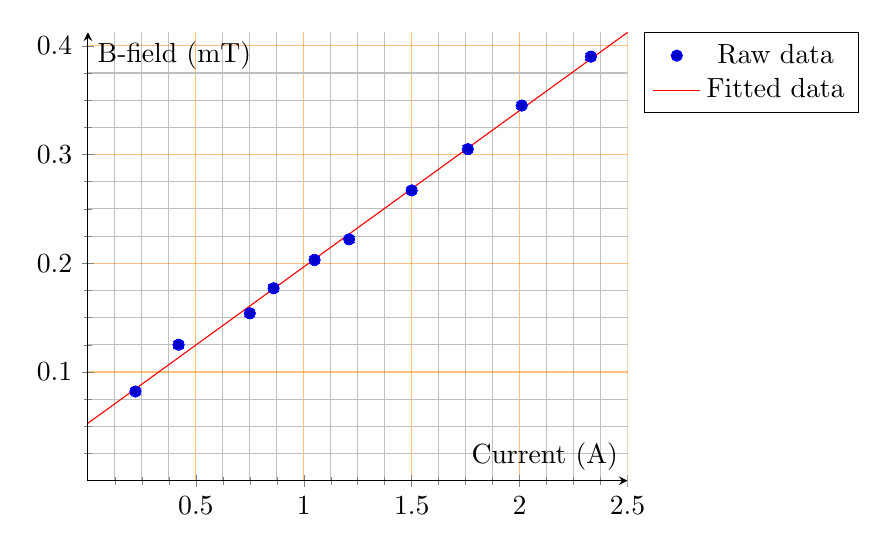
\begin{tikzpicture}
        \begin{axis}[bfield, ymin = 0]
            \addplot +[bfield-scatter] table [
                x error = xerror,
                y error = yerror
            ] {
                x       y       xerror  yerror
                0.22    0.082   0.01    0.003
                0.42    0.125   0.01    0.003
                0.75    0.154   0.01    0.003
                0.86    0.177   0.01    0.003
                1.05    0.203   0.01    0.003
                1.21    0.222   0.01    0.003
                1.50    0.267   0.01    0.003
                1.76    0.305   0.01    0.003
                2.01    0.345   0.01    0.003
                2.33    0.390   0.01    0.003
            };
            \addlegendentry{Raw data}
            
            \addplot +[no marks, domain = 0:2.5] {0.0528311 + 0.143822 * x};
            \addlegendentry{Fitted data}
        \end{axis}
    \end{tikzpicture}
    \caption{Part 3 raw and fitted data (Errors are smaller than point size)}
    \label{fig:part3_graph}
\end{figure}

Figure \ref{fig:part3_graph} shows the raw and fitted data. The linear fit has a gradient of \(\frac{B}{I} = \SI{0.144 \pm 0.005}{\milli\tesla\per\ampere}\).

With our loop density of \(n = \SI{76 \pm 2}{loops per metre}\), solving for \(\mu_0\) gives \SI{1.86 \pm 0.08}{\micro\tesla\metre\per\ampere}.

\section{Discussion}
\subsection{Part 1: The Magnetic Field of the Earth}
Both the calculated and measured inclinations agree with each other, and also with the Australian Geomagnetic Reference Field model's values of \SI{0.0571}{\milli\tesla} at \SI{64.3}{\degree} at Kensington. This indicates our measurement was probably accurate and that the magnetic field probe does not have any significant systematic scale error.

\subsection{Part 2: The Magnetic Field of the Slinky}
As expected, the B-field measured at the ends of the slinky were less than the ones at the middle, due to the field ``spreading out'' at the ends. Compressing the slinky or increasing the current produced a higher B-field strength, also as expected.

The \SI{0.05}{\milli\tesla} variation along the radial distance was much larger than the \SI{0.004}{\milli\tesla} variation along the axis near the middle of the slinky, which could indicate that the loops were too widely spaced to approximate an infinite solenoid well.

Figure \ref{fig:part2_graph} immediately shows that our measured data does not fit the predicted B-field strength. In fact, all but one measurement was greater than the predicted values, which could indicate another source of systematic error that was not accounted for. This may have been simply the slinky not approximating an infinite solenoid well, or it might also have been that the power supply might not have had output a pure DC signal, thus making our predicted values invalid.

\subsection{Part 3: The Permeability of Free Space}
Our result for \(\mu_0\), \SI{1.86 \pm 0.08}{\micro\tesla\metre\per\ampere}, is greater than real value, \SI{1.26}{\micro\tesla\metre\per\ampere}, by \SI{51 \pm 7}{\percent}. This indicates our measured B-field inside the slinky was increasing more than expected per unit current by that percentage.

This result is consistent with the error encountered in part 2, providing more evidence that there was a systematic error involved.

Future experimentation could be to retry the experiment with a higher loop density and placing a capacitor in parallel to the power supply to see if that reduces the systematic error encountered.

\end{document}
